\begin{table*}[t]
\caption{Fresh cases. Absolute outcomes across three generation replicates per bundle. Totals are repeated-condition counts, not independent samples. S and W denote service and wrong-posting loss. B is blocked unresolved requests and U is unstaged failures.}
\centering\small
\begin{tabular}{llrrrrrrrrr}
\toprule
Condition / base & Policy & Loss & Mean & S & W & Correct & Wrong & B & U & Missed \\
\midrule
Correction / 1 & No review & 236 & 9.833 & 132 & 104 & 39 & 12 & 0 & 21 & 12 \\
Correction / 1 & FCFS & 84 & 3.500 & 84 & 0 & 51 & 0 & 0 & 21 & 0 \\
Correction / 1 & EDF & 84 & 3.500 & 84 & 0 & 51 & 0 & 0 & 21 & 0 \\
Correction / 1 & Uncertainty & 84 & 3.500 & 84 & 0 & 51 & 0 & 0 & 21 & 0 \\
Correction / 1 & Greedy & 84 & 3.500 & 84 & 0 & 51 & 0 & 0 & 21 & 0 \\
Correction / 1 & Search & 84 & 3.500 & 84 & 0 & 51 & 0 & 0 & 21 & 0 \\
Correction / 2 & No review & 236 & 9.833 & 132 & 104 & 39 & 12 & 0 & 21 & 12 \\
Correction / 2 & FCFS & 132 & 5.500 & 96 & 36 & 48 & 3 & 0 & 21 & 3 \\
Correction / 2 & EDF & 132 & 5.500 & 96 & 36 & 48 & 3 & 0 & 21 & 3 \\
Correction / 2 & Uncertainty & 84 & 3.500 & 84 & 0 & 51 & 0 & 0 & 21 & 0 \\
Correction / 2 & Greedy & 84 & 3.500 & 84 & 0 & 51 & 0 & 0 & 21 & 0 \\
Correction / 2 & Search & 140 & 5.833 & 100 & 40 & 47 & 4 & 0 & 21 & 4 \\
Approve/block / 1 & No review & 236 & 9.833 & 132 & 104 & 39 & 12 & 0 & 21 & 12 \\
Approve/block / 1 & FCFS & 132 & 5.500 & 132 & 0 & 39 & 0 & 12 & 21 & 0 \\
Approve/block / 1 & EDF & 132 & 5.500 & 132 & 0 & 39 & 0 & 12 & 21 & 0 \\
Approve/block / 1 & Uncertainty & 132 & 5.500 & 132 & 0 & 39 & 0 & 12 & 21 & 0 \\
Approve/block / 1 & Greedy & 132 & 5.500 & 132 & 0 & 39 & 0 & 12 & 21 & 0 \\
Approve/block / 1 & Search & 132 & 5.500 & 132 & 0 & 39 & 0 & 12 & 21 & 0 \\
Approve/block / 2 & No review & 236 & 9.833 & 132 & 104 & 39 & 12 & 0 & 21 & 12 \\
Approve/block / 2 & FCFS & 168 & 7.000 & 132 & 36 & 39 & 3 & 9 & 21 & 3 \\
Approve/block / 2 & EDF & 168 & 7.000 & 132 & 36 & 39 & 3 & 9 & 21 & 3 \\
Approve/block / 2 & Uncertainty & 132 & 5.500 & 132 & 0 & 39 & 0 & 12 & 21 & 0 \\
Approve/block / 2 & Greedy & 132 & 5.500 & 132 & 0 & 39 & 0 & 12 & 21 & 0 \\
Approve/block / 2 & Search & 172 & 7.167 & 132 & 40 & 39 & 4 & 8 & 21 & 4 \\
Complexity time / 1 & No review & 236 & 9.833 & 132 & 104 & 39 & 12 & 0 & 21 & 12 \\
Complexity time / 1 & FCFS & 84 & 3.500 & 84 & 0 & 51 & 0 & 0 & 21 & 0 \\
Complexity time / 1 & EDF & 84 & 3.500 & 84 & 0 & 51 & 0 & 0 & 21 & 0 \\
Complexity time / 1 & Uncertainty & 84 & 3.500 & 84 & 0 & 51 & 0 & 0 & 21 & 0 \\
Complexity time / 1 & Greedy & 84 & 3.500 & 84 & 0 & 51 & 0 & 0 & 21 & 0 \\
Complexity time / 1 & Search & 84 & 3.500 & 84 & 0 & 51 & 0 & 0 & 21 & 0 \\
Complexity time / 2 & No review & 236 & 9.833 & 132 & 104 & 39 & 12 & 0 & 21 & 12 \\
Complexity time / 2 & FCFS & 140 & 5.833 & 100 & 40 & 47 & 4 & 0 & 21 & 4 \\
Complexity time / 2 & EDF & 140 & 5.833 & 100 & 40 & 47 & 4 & 0 & 21 & 4 \\
Complexity time / 2 & Uncertainty & 92 & 3.833 & 88 & 4 & 50 & 1 & 0 & 21 & 1 \\
Complexity time / 2 & Greedy & 92 & 3.833 & 88 & 4 & 50 & 1 & 0 & 21 & 1 \\
Complexity time / 2 & Search & 148 & 6.167 & 104 & 44 & 46 & 5 & 0 & 21 & 5 \\
\bottomrule
\end{tabular}
\end{table*}

\begin{table*}[t]
\caption{Fresh cases. Review resources. Time and waiting are summed abstract ticks. Utilization is mean occupied fraction of the processing horizon. More reviews do not necessarily imply more useful interventions.}
\centering\small
\begin{tabular}{llrrrrrr}
\toprule
Condition / base & Policy & Reviews & Corrections & Time & Waiting & Utilization & Multi-eligible \\
\midrule
Correction / 1 & No review & 0 & 0 & 0 & 0 & 0.000 & 57 \\
Correction / 1 & FCFS & 51 & 12 & 51 & 19 & 0.401 & 19 \\
Correction / 1 & EDF & 51 & 12 & 51 & 19 & 0.401 & 19 \\
Correction / 1 & Uncertainty & 46 & 12 & 46 & 9 & 0.361 & 19 \\
Correction / 1 & Greedy & 46 & 12 & 46 & 9 & 0.361 & 19 \\
Correction / 1 & Search & 51 & 12 & 51 & 19 & 0.401 & 19 \\
Correction / 2 & No review & 0 & 0 & 0 & 0 & 0.000 & 38 \\
Correction / 2 & FCFS & 44 & 9 & 88 & 32 & 0.686 & 18 \\
Correction / 2 & EDF & 44 & 9 & 88 & 33 & 0.686 & 19 \\
Correction / 2 & Uncertainty & 42 & 12 & 84 & 23 & 0.658 & 14 \\
Correction / 2 & Greedy & 42 & 12 & 84 & 23 & 0.658 & 14 \\
Correction / 2 & Search & 44 & 8 & 88 & 32 & 0.686 & 19 \\
Approve/block / 1 & No review & 0 & 0 & 0 & 0 & 0.000 & 57 \\
Approve/block / 1 & FCFS & 51 & 0 & 51 & 19 & 0.401 & 19 \\
Approve/block / 1 & EDF & 51 & 0 & 51 & 19 & 0.401 & 19 \\
Approve/block / 1 & Uncertainty & 46 & 0 & 46 & 9 & 0.361 & 19 \\
Approve/block / 1 & Greedy & 46 & 0 & 46 & 9 & 0.361 & 19 \\
Approve/block / 1 & Search & 51 & 0 & 51 & 19 & 0.401 & 19 \\
Approve/block / 2 & No review & 0 & 0 & 0 & 0 & 0.000 & 38 \\
Approve/block / 2 & FCFS & 44 & 0 & 88 & 32 & 0.686 & 18 \\
Approve/block / 2 & EDF & 44 & 0 & 88 & 33 & 0.686 & 19 \\
Approve/block / 2 & Uncertainty & 42 & 0 & 84 & 23 & 0.658 & 14 \\
Approve/block / 2 & Greedy & 42 & 0 & 84 & 23 & 0.658 & 14 \\
Approve/block / 2 & Search & 44 & 0 & 88 & 32 & 0.686 & 19 \\
Complexity time / 1 & No review & 0 & 0 & 0 & 0 & 0.000 & 52 \\
Complexity time / 1 & FCFS & 50 & 12 & 56 & 22 & 0.442 & 18 \\
Complexity time / 1 & EDF & 51 & 12 & 57 & 24 & 0.450 & 19 \\
Complexity time / 1 & Uncertainty & 46 & 12 & 52 & 14 & 0.410 & 15 \\
Complexity time / 1 & Greedy & 46 & 12 & 52 & 14 & 0.410 & 15 \\
Complexity time / 1 & Search & 51 & 12 & 57 & 24 & 0.450 & 19 \\
Complexity time / 2 & No review & 0 & 0 & 0 & 0 & 0.000 & 34 \\
Complexity time / 2 & FCFS & 43 & 8 & 91 & 32 & 0.714 & 18 \\
Complexity time / 2 & EDF & 43 & 8 & 91 & 32 & 0.714 & 19 \\
Complexity time / 2 & Uncertainty & 41 & 11 & 87 & 26 & 0.686 & 14 \\
Complexity time / 2 & Greedy & 41 & 11 & 87 & 26 & 0.686 & 14 \\
Complexity time / 2 & Search & 43 & 7 & 90 & 31 & 0.706 & 19 \\
\bottomrule
\end{tabular}
\end{table*}

\begin{table*}[t]
\caption{Fresh cases. Search-minus-comparator loss differences. Negative favors search. Intervals resample bundles; W/T/L are scenario-bundle wins, ties and losses. Only the fresh approve/block two-tick search--greedy row is primary.}
\centering\small
\begin{tabular}{llrrll}
\toprule
Condition & Comparator & Base & Difference & 95\% interval & W/T/L \\
\midrule
Correction & greedy & 1 & 0.000 & [0.000, 0.000] & 0/8/0 \\
Correction & edf & 1 & 0.000 & [0.000, 0.000] & 0/8/0 \\
Correction & greedy & 2 & 2.333 & [0.000, 6.333] & 0/6/2 \\
Correction & edf & 2 & 0.333 & [0.000, 1.000] & 0/7/1 \\
Approve/block & greedy & 1 & 0.000 & [0.000, 0.000] & 0/8/0 \\
Approve/block & edf & 1 & 0.000 & [0.000, 0.000] & 0/8/0 \\
Approve/block & greedy & 2 & 1.667 & [0.000, 4.667] & 0/6/2 \\
Approve/block & edf & 2 & 0.167 & [0.000, 0.500] & 0/7/1 \\
Complexity time & greedy & 1 & 0.000 & [0.000, 0.000] & 0/8/0 \\
Complexity time & edf & 1 & 0.000 & [0.000, 0.000] & 0/8/0 \\
Complexity time & greedy & 2 & 2.333 & [0.000, 6.333] & 0/6/2 \\
Complexity time & edf & 2 & 0.333 & [0.000, 1.000] & 0/7/1 \\
\bottomrule
\end{tabular}
\end{table*}

\begin{table*}[t]
\caption{Post hoc Stage 5 preparations. Absolute outcomes across three generation replicates per bundle. Totals are repeated-condition counts, not independent samples. S and W denote service and wrong-posting loss. B is blocked unresolved requests and U is unstaged failures.}
\centering\small
\begin{tabular}{llrrrrrrrrr}
\toprule
Condition / base & Policy & Loss & Mean & S & W & Correct & Wrong & B & U & Missed \\
\midrule
Correction / 1 & No review & 800 & 8.333 & 424 & 376 & 182 & 51 & 0 & 55 & 51 \\
Correction / 1 & FCFS & 220 & 2.292 & 220 & 0 & 233 & 0 & 0 & 55 & 0 \\
Correction / 1 & EDF & 220 & 2.292 & 220 & 0 & 233 & 0 & 0 & 55 & 0 \\
Correction / 1 & Uncertainty & 220 & 2.292 & 220 & 0 & 233 & 0 & 0 & 55 & 0 \\
Correction / 1 & Greedy & 220 & 2.292 & 220 & 0 & 233 & 0 & 0 & 55 & 0 \\
Correction / 1 & Search & 220 & 2.292 & 220 & 0 & 233 & 0 & 0 & 55 & 0 \\
Correction / 2 & No review & 800 & 8.333 & 424 & 376 & 182 & 51 & 0 & 55 & 51 \\
Correction / 2 & FCFS & 480 & 5.000 & 312 & 168 & 210 & 23 & 0 & 55 & 23 \\
Correction / 2 & EDF & 440 & 4.583 & 292 & 148 & 215 & 18 & 0 & 55 & 18 \\
Correction / 2 & Uncertainty & 332 & 3.458 & 260 & 72 & 223 & 10 & 0 & 55 & 10 \\
Correction / 2 & Greedy & 332 & 3.458 & 260 & 72 & 223 & 10 & 0 & 55 & 10 \\
Correction / 2 & Search & 356 & 3.708 & 264 & 92 & 222 & 11 & 0 & 55 & 11 \\
Approve/block / 1 & No review & 800 & 8.333 & 424 & 376 & 182 & 51 & 0 & 55 & 51 \\
Approve/block / 1 & FCFS & 424 & 4.417 & 424 & 0 & 182 & 0 & 51 & 55 & 0 \\
Approve/block / 1 & EDF & 424 & 4.417 & 424 & 0 & 182 & 0 & 51 & 55 & 0 \\
Approve/block / 1 & Uncertainty & 424 & 4.417 & 424 & 0 & 182 & 0 & 51 & 55 & 0 \\
Approve/block / 1 & Greedy & 424 & 4.417 & 424 & 0 & 182 & 0 & 51 & 55 & 0 \\
Approve/block / 1 & Search & 424 & 4.417 & 424 & 0 & 182 & 0 & 51 & 55 & 0 \\
Approve/block / 2 & No review & 800 & 8.333 & 424 & 376 & 182 & 51 & 0 & 55 & 51 \\
Approve/block / 2 & FCFS & 592 & 6.167 & 424 & 168 & 182 & 23 & 28 & 55 & 23 \\
Approve/block / 2 & EDF & 572 & 5.958 & 424 & 148 & 182 & 18 & 33 & 55 & 18 \\
Approve/block / 2 & Uncertainty & 496 & 5.167 & 424 & 72 & 182 & 10 & 41 & 55 & 10 \\
Approve/block / 2 & Greedy & 496 & 5.167 & 424 & 72 & 182 & 10 & 41 & 55 & 10 \\
Approve/block / 2 & Search & 508 & 5.292 & 424 & 84 & 182 & 11 & 40 & 55 & 11 \\
Complexity time / 1 & No review & 800 & 8.333 & 424 & 376 & 182 & 51 & 0 & 55 & 51 \\
Complexity time / 1 & FCFS & 284 & 2.958 & 240 & 44 & 228 & 5 & 0 & 55 & 5 \\
Complexity time / 1 & EDF & 220 & 2.292 & 220 & 0 & 233 & 0 & 0 & 55 & 0 \\
Complexity time / 1 & Uncertainty & 244 & 2.542 & 228 & 16 & 231 & 2 & 0 & 55 & 2 \\
Complexity time / 1 & Greedy & 244 & 2.542 & 228 & 16 & 231 & 2 & 0 & 55 & 2 \\
Complexity time / 1 & Search & 236 & 2.458 & 224 & 12 & 232 & 1 & 0 & 55 & 1 \\
Complexity time / 2 & No review & 800 & 8.333 & 424 & 376 & 182 & 51 & 0 & 55 & 51 \\
Complexity time / 2 & FCFS & 512 & 5.333 & 324 & 188 & 207 & 26 & 0 & 55 & 26 \\
Complexity time / 2 & EDF & 464 & 4.833 & 300 & 164 & 213 & 20 & 0 & 55 & 20 \\
Complexity time / 2 & Uncertainty & 332 & 3.458 & 260 & 72 & 223 & 10 & 0 & 55 & 10 \\
Complexity time / 2 & Greedy & 332 & 3.458 & 260 & 72 & 223 & 10 & 0 & 55 & 10 \\
Complexity time / 2 & Search & 380 & 3.958 & 272 & 108 & 220 & 13 & 0 & 55 & 13 \\
\bottomrule
\end{tabular}
\end{table*}

\begin{table*}[t]
\caption{Post hoc Stage 5 preparations. Review resources. Time and waiting are summed abstract ticks. Utilization is mean occupied fraction of the processing horizon. More reviews do not necessarily imply more useful interventions.}
\centering\small
\begin{tabular}{llrrrrrr}
\toprule
Condition / base & Policy & Reviews & Corrections & Time & Waiting & Utilization & Multi-eligible \\
\midrule
Correction / 1 & No review & 0 & 0 & 0 & 0 & 0.000 & 301 \\
Correction / 1 & FCFS & 233 & 51 & 233 & 115 & 0.459 & 115 \\
Correction / 1 & EDF & 233 & 51 & 233 & 115 & 0.459 & 115 \\
Correction / 1 & Uncertainty & 224 & 51 & 224 & 97 & 0.442 & 115 \\
Correction / 1 & Greedy & 224 & 51 & 224 & 97 & 0.442 & 115 \\
Correction / 1 & Search & 233 & 51 & 233 & 115 & 0.459 & 115 \\
Correction / 2 & No review & 0 & 0 & 0 & 0 & 0.000 & 212 \\
Correction / 2 & FCFS & 182 & 28 & 364 & 152 & 0.712 & 87 \\
Correction / 2 & EDF & 190 & 33 & 380 & 191 & 0.740 & 103 \\
Correction / 2 & Uncertainty & 169 & 41 & 338 & 104 & 0.664 & 83 \\
Correction / 2 & Greedy & 169 & 41 & 338 & 104 & 0.664 & 83 \\
Correction / 2 & Search & 190 & 40 & 380 & 184 & 0.740 & 103 \\
Approve/block / 1 & No review & 0 & 0 & 0 & 0 & 0.000 & 301 \\
Approve/block / 1 & FCFS & 233 & 0 & 233 & 115 & 0.459 & 115 \\
Approve/block / 1 & EDF & 233 & 0 & 233 & 115 & 0.459 & 115 \\
Approve/block / 1 & Uncertainty & 224 & 0 & 224 & 97 & 0.442 & 115 \\
Approve/block / 1 & Greedy & 224 & 0 & 224 & 97 & 0.442 & 115 \\
Approve/block / 1 & Search & 233 & 0 & 233 & 115 & 0.459 & 115 \\
Approve/block / 2 & No review & 0 & 0 & 0 & 0 & 0.000 & 212 \\
Approve/block / 2 & FCFS & 182 & 0 & 364 & 152 & 0.712 & 87 \\
Approve/block / 2 & EDF & 190 & 0 & 380 & 191 & 0.740 & 103 \\
Approve/block / 2 & Uncertainty & 169 & 0 & 338 & 104 & 0.664 & 83 \\
Approve/block / 2 & Greedy & 169 & 0 & 338 & 104 & 0.664 & 83 \\
Approve/block / 2 & Search & 190 & 0 & 380 & 182 & 0.740 & 103 \\
Complexity time / 1 & No review & 0 & 0 & 0 & 0 & 0.000 & 290 \\
Complexity time / 1 & FCFS & 219 & 46 & 239 & 107 & 0.472 & 106 \\
Complexity time / 1 & EDF & 233 & 51 & 256 & 133 & 0.506 & 115 \\
Complexity time / 1 & Uncertainty & 216 & 49 & 237 & 104 & 0.467 & 109 \\
Complexity time / 1 & Greedy & 216 & 49 & 237 & 104 & 0.467 & 109 \\
Complexity time / 1 & Search & 232 & 50 & 254 & 132 & 0.502 & 114 \\
Complexity time / 2 & No review & 0 & 0 & 0 & 0 & 0.000 & 200 \\
Complexity time / 2 & FCFS & 175 & 25 & 365 & 144 & 0.714 & 86 \\
Complexity time / 2 & EDF & 186 & 31 & 386 & 177 & 0.755 & 98 \\
Complexity time / 2 & Uncertainty & 161 & 41 & 337 & 88 & 0.664 & 79 \\
Complexity time / 2 & Greedy & 161 & 41 & 337 & 88 & 0.664 & 79 \\
Complexity time / 2 & Search & 186 & 38 & 386 & 170 & 0.755 & 98 \\
\bottomrule
\end{tabular}
\end{table*}

\begin{table*}[t]
\caption{Post hoc Stage 5 preparations. Search-minus-comparator loss differences. Negative favors search. Intervals resample bundles; W/T/L are scenario-bundle wins, ties and losses. Only the fresh approve/block two-tick search--greedy row is primary.}
\centering\small
\begin{tabular}{llrrll}
\toprule
Condition & Comparator & Base & Difference & 95\% interval & W/T/L \\
\midrule
Correction & greedy & 1 & 0.000 & [0.000, 0.000] & 0/32/0 \\
Correction & edf & 1 & 0.000 & [0.000, 0.000] & 0/32/0 \\
Correction & greedy & 2 & 0.250 & [-0.333, 0.917] & 1/29/2 \\
Correction & edf & 2 & -0.875 & [-2.000, 0.000] & 3/29/0 \\
Approve/block & greedy & 1 & 0.000 & [0.000, 0.000] & 0/32/0 \\
Approve/block & edf & 1 & 0.000 & [0.000, 0.000] & 0/32/0 \\
Approve/block & greedy & 2 & 0.125 & [-0.167, 0.500] & 1/29/2 \\
Approve/block & edf & 2 & -0.667 & [-1.417, -0.083] & 4/28/0 \\
Complexity time & greedy & 1 & -0.083 & [-0.250, 0.000] & 1/31/0 \\
Complexity time & edf & 1 & 0.167 & [0.000, 0.500] & 0/31/1 \\
Complexity time & greedy & 2 & 0.500 & [-0.083, 1.250] & 1/28/3 \\
Complexity time & edf & 2 & -0.875 & [-2.000, 0.000] & 3/29/0 \\
\bottomrule
\end{tabular}
\end{table*}

\begin{figure*}[t]
\centering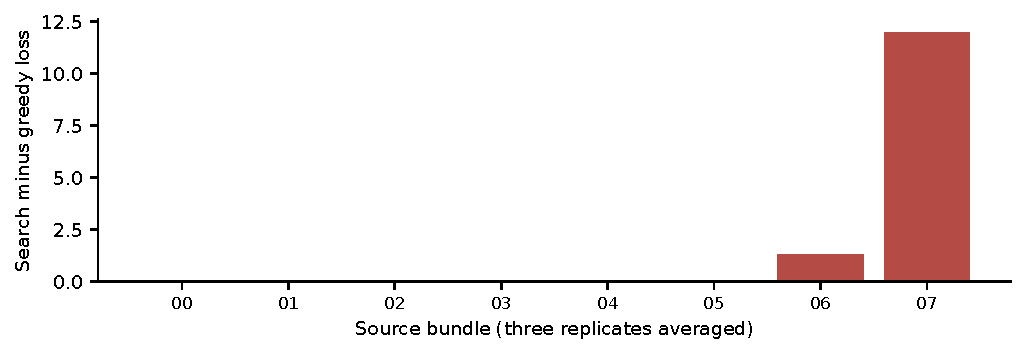
\includegraphics[width=0.98\textwidth]{../artifacts/stage6_robustness/analysis/fresh/figures/primary_bundle_differences.pdf}
\caption{All eight fresh primary bundle differences, after averaging three generation replicates. Zero values remain explicit.}
\end{figure*}
\begin{figure*}[t]
\centering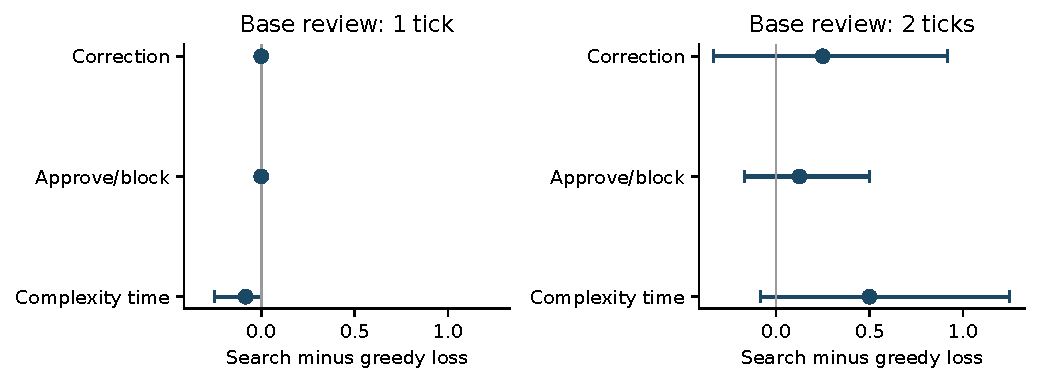
\includegraphics[width=0.98\textwidth]{../artifacts/stage6_robustness/analysis/post_hoc_stage5/figures/paired_loss.pdf}
\caption{Post hoc saved-preparation sensitivity. The 32 bundles are separate from the eight fresh bundles and are not pooled for inference.}
\end{figure*}
